\documentclass[sigplan,screen]{acmart}\settopmatter{printfolios=true,printccs=false,printacmref=false}
%\documentclass[acmsmall,review,anonymous]{acmart}\settopmatter{printfolios=true,printccs=false,printacmref=false}

\usepackage[utf8]{inputenc}
\usepackage[T1]{fontenc}

\usepackage{adjustbox}
\usepackage{booktabs}
\usepackage{listings}
\usepackage{multicol}
\usepackage[autolanguage]{numprint}
\usepackage{proof}
\usepackage{softdev}
\usepackage{stmaryrd}
\usepackage{subcaption}
\usepackage{wrapfig}
\usepackage{xspace}
\usepackage{menukeys}

\usepackage[ruled]{algorithm2e} % For algorithms
\renewcommand{\algorithmcfname}{ALGORITHM}
\SetAlFnt{\small}
\SetAlCapFnt{\small}
\SetAlCapNameFnt{\small}
\SetAlCapHSkip{0pt}
\IncMargin{-\parindent}

%\acmJournal{SLE}
%\acmVolume{1}
%\acmNumber{CONF} % CONF = POPL or ICFP or OOPSLA
%\acmArticle{1}
%\acmYear{2019}
%\acmMonth{1}
%\acmDOI{} % \acmDOI{10.1145/nnnnnnn.nnnnnnn}
\acmConference[SLE'19]{Software Language Engineering}{October 2019}{Athens, Greece}
\startPage{1}

\lstset{
    basicstyle=\ttfamily\scriptsize,
    xleftmargin=0pt,
    numbersep=.8em,
    numberstyle=\scriptsize\tt\color{gray},
    captionpos=b,
    escapeinside={{<!}{!>}},
}

% from https://tex.stackexchange.com/questions/264361/skipping-line-numbers-in-lstlisting#264373
\let\origthelstnumber\thelstnumber
\makeatletter
\newcommand*\Suppressnumber{%
  \lst@AddToHook{OnNewLine}{%
    \let\thelstnumber\relax%
     \advance\c@lstnumber-\@ne\relax%
    }%
}

\newcommand*\Reactivatenumber[1]{%
  \setcounter{lstnumber}{\numexpr#1-1\relax}
  \lst@AddToHook{OnNewLine}{%
   \let\thelstnumber\origthelstnumber%
   \refstepcounter{lstnumber}
  }%
}

\setcopyright{none}

\bibliographystyle{ACM-Reference-Format}
\citestyle{acmauthoryear}

% DOI
%\acmDOI{0000001.0000001}

% Paper history
%\received{February 2007}

\newcommand{\inputtree}[0]{\emph{CST}\xspace}
\newcommand{\eco}[0]{\emph{Eco}\xspace}
\newcommand{\ald}[0]{\emph{ALD}\xspace}
\newcommand{\qtt}[1]{`\texttt{#1}'\xspace}

\newcommand{\hotkeynewlbox}[0]{\keys{Ctrl+L}\xspace}
\newcommand{\hotkeyleavelbox}[0]{\keys{Ctrl+Shift+L}\xspace}

\lstnewenvironment{lstdefault}[1][]
  {
    \lstset{
        numbers=left,
        language=Python,
        keywordstyle=\color{red!70!black},
        commentstyle=\itshape\color{gray!90!black},
        stringstyle=\color{green!60!black},
        basicstyle=\linespread{1.0}\footnotesize\ttfamily,
        numberstyle=\tiny,
        keepspaces=true,
        breaklines=true,
        captionpos=b,
        abovecaptionskip=0.8em,
        columns=fullflexible,
        xleftmargin=10pt,
        aboveskip=1em,
        belowskip=0em,
        showstringspaces=false,
        literate={\$}{{\$}}1,
        escapeinside={{<!}{!>}},
        #1
    }
}{}

\lstdefinelanguage{EcoGrammar}
{
    alsoletter={:,\:=,|},
    morekeywords={:, =, | },
    keywordstyle=\color{red!70!black},
    morestring=[b]",
    stringstyle=\color{green!60!black},
    commentstyle=\itshape\color{gray!90!black},
    comment=[l]{//},
    morecomment=[s]{/*}{*/},
}

\lstnewenvironment{lsteco}[1][]
  {
    \lstset{
        language=EcoGrammar,
        basicstyle=\footnotesize\ttfamily,
        numberstyle=\tiny,
        xleftmargin=10pt,
        showstringspaces=false,
        #1
    }
}{}

% Document starts
\begin{document}
% Title portion. Note the short title for running heads
\title{Automatic Language boxes}

\author{Lukas Diekmann}
\affiliation{%
  \department{Software Development Team}
  \institution{King's College London}
  \country{United Kingdom}}
\author{Laurence Tratt}
\orcid{0000-0002-5258-3805}
\affiliation{%
  \department{Software Development Team}
  \institution{King's College London}
  \country{United Kingdom}
}
\thanks{Authors' URLs: %
    L.~Diekmann~\url{http://lukasdiekmann.com/},
    L.~Tratt~\url{http://tratt.net/laurie/}.
}


\begin{abstract}
Since composed grammars are often ambiguous, grammar composition requires a
mechanism for dealing with ambiguity: either ruling it out entirely through the use of
delimiters, or by selecting the desired parse tree from the parse forest.  In
this paper we show that \emph{language boxes} -- a delimiter-based
mechanism atop incremental parsing -- can be extended in a way that fits
between these two extremes. In essence, we retain the use of delimiters, but
when errors appear in the user's input, we selectively reparse the user's
input, taking into account the user's editor history, and insert, remove,
or move delimiters -- leading to what we call \emph{automatic language
boxes}. The very nature of the problem means that automatic language boxes
cannot always match a user's intention: rather, our aim is to find a simple
heuristic that does the right thing in most cases, while rarely surprising the
user when it cannot. Our case studies show that \laurie{XXX}.
\end{abstract}

\keywords{Parsing, language composition, programming languages}

\maketitle

\section{Introduction}

Language composition -- the ability to build larger languages out of multiple
small languages -- offers an enticing solution to problems such as the
development of domain-specific languages or the migration of legacy software.
Unfortunately, writing and editing composed programs is often cumbersome.
The basic problem is that grammar
composition -- which underpins language composition -- can cause
two provably unambiguous grammars to become ambiguous when composed,
and determining whether a grammar is unambiguous or not is
undecidable~\cite{cantor62ambiguity}. There are two fundamental approaches
of coping with ambiguity: either ruling it out through the use of
delimiters (either via explicit bracketing or syntax-directed
editing); or to use a generalised parsing algorithm that can cope with ambiguity
(e.g.~\cite{visser97scannerless}). Each has different trade-offs: delimiters
are visually intrusive and/or awkward to work with; and one can never know if all possible
ambiguous parses have been covered by disambiguation operators.

An alternative to traditional delimiter-based approaches are \emph{language boxes} which aim to
combine the advantages of explicit bracketing and syntax-based
editing without the disadvantages~\cite{diekmann14eco}. Building atop the
incremental parsing algorithm
of \citet{wagner98practicalalgorithms}, language boxes are nodes in the parse
tree that represent a different language: the language box is surrounded by
explicit, but invisible, delimiters. Unlike explicit bracketing approaches,
there are no visually intrusive delimiters; unlike traditional
syntax-based editors, the program can be syntactically incorrect in arbitrary
ways and places during editing. However, language boxes lack the most appealing aspect of
ambiguous parsing: users must explicitly, and tediously, state when they want
to insert language boxes.

The fundamental research question underlying this paper is whether it is
possible to reduce the need for the users to explicitly insert language
boxes. For example, in a composition of Java and SQL (where SQL is allowed
wherever a Java expression is valid), can such a system automatically insert an
SQL language box for the input \texttt{for (String n: SELECT name FROM table) \{ ...
\}}? It is important to acknowledge from the outset that a `perfect' solution
is impossible, since there will always be some cases where there are multiple
ways of splitting the same input across different language boxes. Realistic
solutions must also take into account other considerations: it should not
require significant extra work for the authors of composed languages; performance must
not be unduly impacted; and users should be able to broadly predict if, and
why, language boxes are inserted or not.

The solution we present to this problem are \emph{automatic language boxes}. In
essence, we present a heuristic which can insert, remove, and update language
boxes in many useful cases. The heuristic is triggered only when there is a
syntax error in the input of the language the user is currently typing in
(making it fairly predictable). When an error does occur, text is selectively
reparsed to see if inserting or removing language boxes would fix the error
(in general leading to only a small performance overhead, though some
compositions can hit worse cases). One of the main challenges is
to determine what text to reparse: we present several sub-heuristics (including
the ability to take the user's previous input into consideration) which, when
combined, lead to an effective heuristic for many cases (see Figure \ref{intro_example} for an example).

\begin{figure}
    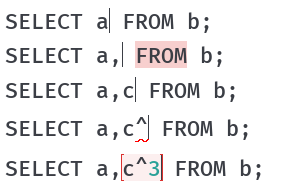
\includegraphics[width=0.3\textwidth]{images/auto_remove_insert_sql_java}
    \caption{\laurie{we need to add line numbers or a) b) c) annotations to the side (in \LaTeX, not in the image)}Automatic language boxes in action with a composition of SQL
      and Java, where Java expressions can be used wherever SQL expressions
      are valid. The initial input is \texttt{SELECT a FROM b;}, with the user
      putting their cursor immediately after `\texttt{a}' and typing `\texttt{,c\^3}'.
    The user starts with a valid SQLite program. \textbf{b)} After typing
    `\texttt{,}' an error occurs which is fixed by automatically wrapping
    `\texttt{FROM}' inside a Java language box.  \textbf{c)} After typing
    `\texttt{c}' the language box is removed again, since `\texttt{FROM}' is
    valid in the outer language again. Typing `\texttt{\textasciicircum3}' produces an error
    which is fixed by wrapping the expression `\texttt{c\textasciicircum3}' inside a Java
    language box.
}
\label{intro_example}
\end{figure}

\laurie{this needs revisiting}The paper is structured as follows: Section \ref{sec_background} gives an
overview on incremental lexing and parsing as well as language composition
using language boxes. Section \ref{sec_finding_lbox_candidates}
describes how we can use parsing errors to find automatic language boxes, how
we can present multiple solutions to the user, and how automatically inserted
language boxes can also automatically be removed again. Section
\ref{sec_lbox_limitations} describes some of the limitations of automatic
language boxes, e.g.~where either unwanted language boxes are inserted or
detection fails and no language box is inserted at all. Section
\ref{sec:impl_defaultrec} describes the implementation of recognisers, which
are used during the detection of automatic language boxes.



\section{Background}
\label{sec_background}

In this section, we briefly survey existing approaches to editing composed
programs, before giving a brief overview of incremental parsing, sufficient for
this paper's purposes.

\subsection{Explicit delimiter approaches}

The traditional approach to language composition is to use delimiters
to make clear when the user has switched from one sub-language to another. The
most obvious way of achieving this is to use explicit brackets to make clear a
switch from an outer to an inner language (e.g.~\texttt{for (String e: <<SELECT name
FROM table>>) \{ ... \}}), though this is visually intrusive, and prevents the
special brackets being used within the sub-language (e.g.~in this case, the sub language
cannot use `>>' as a bit-wise operator).

Naive approaches inherit a severe restriction from traditional parsing, which
separates lexing (i.e.~the splitting of the user's input into tokens) from
parsing (i.e.~the structuring of tokens into a parse tree): all the languages
must share the same lexing rules. This restriction can be somewhat eased if the
lexer recognises the explicit brackets and extracts text between them wholesale
for separate lexing and parsing (see e.g.~\cite[p.~13-14]{tratt08domain}),
though it is then hard for the lexer to accurately keep track of nested special
brackets (e.g.~should brackets in comments be counted or not?).  A
more sophisticated approach is for the lexer and parser to interact (see
e.g.~\cite{wyk07context}), such that the parse causes a switch in lexing rules
when input shifts to an inner language.
This has the advantage that brackets do not always need to be quite as visually
intrusive (e.g.~if an inner language has different keywords to the outer
language, that can be used to indicate the switch from one language to
another), though in the general case explicit brackets must still be
used to resolve ambiguities.


\subsection{Scannerless parsing}

Generalised parsing can parse any Context-Free Grammar (CFG), even those that
are ambiguous. Scannerless parsing~\cite{visser97scannerless} extends this such
that lexing and parsing are specified together. This removes the need for
special brackets entirely, but does so at the expense of causing many more
ambiguities (since traditional lexers implicitly resolve many ambiguities, such
as between identifiers and keywords, before parsing).
This is challenging because ambiguity is, in general,
undecidable~\cite{cantor62ambiguity} and even the best ambiguity heuristics fail
to find all possible sources of ambiguity~\cite{vasudevan13detecting}. Thus,
no matter how many static disambiguation operators one uses, in general one
cannot be sure if all possible points of ambiguity have been covered.
Furthermore, our current disambiguation operators can cause scannerless
parsers to become context-sensitive~\cite{eijck__lets_accept_rejects}, the
consequences of which are still unclear.


\subsection{Syntax directed editing}

Traditional syntax directed editing avoids parsing text entirely. In essence,
users edit an AST directly, with uncompleted parts of a program being
represented by holes. This avoids the need for explicit delimiters, and
sidesteps issues of ambiguity completely. However, such systems are awkward to
use\cite[p.~2]{khwaja93syntax}, for example only allowing whole nodes in the AST to be selected at a time,
and quickly fell out of fashion. The modern syntax directed editor
MPS~\cite{pech13mps} alleviates some, though not all, of these problems;
however, it requires significant expertise on the part of the composition author to make
editing a pleasant experience.


\subsection{Incremental parsing}

Parsing is traditionally a batch process: an entire file is fed through a parser
and a parse tree is created from it. Incremental parsing, in contrast,
continually parses text as the user types and
updates a parse tree. In this paper we make use of the incremental lexing and
LR incremental parsing algorithms of~\citet{wagner98practicalalgorithms}
\laurie{we should add a footnote here along the lines of ``Taking into account
the fixes from Lukas'd Phd thesis [cite]``}: it handles the full class of
$\textrm{LR}(k)$ grammars; and has
formal guarantees that the algorithm is optimal (i.e.~the number of steps
needed to integrate user changes into an existing parse tree is minimal).
Furthermore, Wagner presents an algorithm for incremental lexical analysis,
improving on works such as \cite{fischer84poe, bahlke86psg, ballance92pan,
fischer92aladin}. The following gives a brief overview of incremental lexing
and parsing.

An incremental parser and lexer both operate on a parse tree. Parse tree nodes
are either \emph{nonterminals} (representing rules in the grammar) or
\emph{tokens} (representing terminal symbols). Nonterminal nodes are immutable
(i.e.~their type cannot change) and have zero or more ordered child nodes
(which are not immutable and can be updated). Tokens have a type (e.g.~`int')
and a value (e.g.~`3') and are mutable. Figure \ref{fig_example_parsetree}
shows an example of a parse tree.

\begin{figure}
\begin{minipage}[b]{0.17\textwidth}
\begin{lsteco}
// Parser
Var: Id "eq" Val;
Id: "id";
Val: "int";

// Lexer
eq:"="
id:"[a-z]+"
int:"[0-9]+"
\end{lsteco}
\end{minipage}
\begin{minipage}[b]{0.30\textwidth}
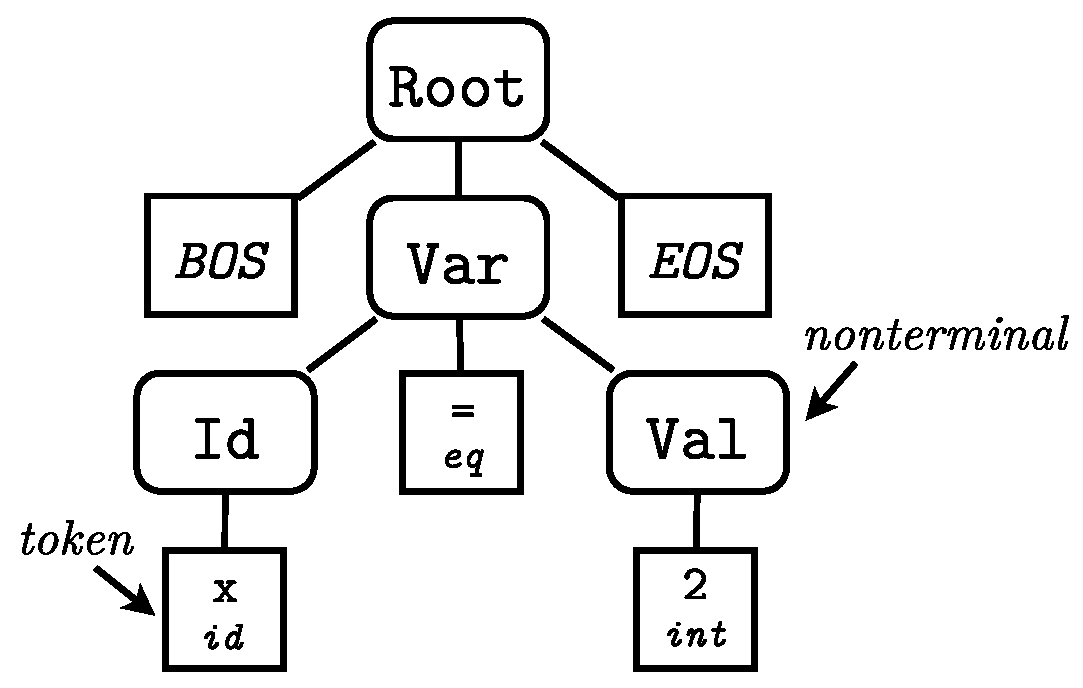
\includegraphics[width=1.0\textwidth]{images/sampleparsetree}
\end{minipage}
\caption{An example of a parse tree constructed from the grammar on the left.
The minimal parse tree consists of three
special nodes: a \emph{Root} nonterminal; and \emph{BOS} (Beginning of
Stream) and \emph{EOS} (End of Stream) terminals (both children of
\emph{Root}). For brevity reasons, these nodes are elided for the remainder of
this thesis. All nodes created from user input are (directly or indirectly)
children of \emph{Root} and are contained between \emph{BOS} and \emph{EOS}.}
\label{fig_example_parsetree}
\end{figure}

When the user types, the incremental lexer first either creates, or updates,
tokens in the parse tree. The lexer considers where the cursor is in the tree
(i.e.~where the user is typing) and uses lookahead knowledge stored in the
tokens to work out the affected area of the change. Newly created tokens are
then merged back into the tree.  In the simple case where a token's value, but
not its type, was changed, no further action is needed. In all other cases, the
path from each changed token up to the root is first marked with \textit{nested
change} flags which are then used by the incremental parser to update the parse
tree. The incremental parser starts at the beginning of the tree and tries to
reparse all subtrees that contain changes. Assuming the user's input is
syntactically valid, nonterminals are created or removed, as appropriate.
Unchanged subtrees are reused as is whenever possible. Since nonterminals are
immutable, subtrees which can't be reused must be recreated from scratch.

Syntactically incomplete programs lead to temporarily incorrect parse trees.
In such cases, the incremental parser typically attaches tokens to a single
parent. When the user eventually creates a syntactically valid program, the
tree is rewritten.

\subsection{Language boxes}

Language boxes allow users to embed one language inside another.  Language
boxes have a type (e.g.~HTML), an associated editor (e.g.~an extended
incremental parser), and a value (e.g.~a parse tree).  By design, language
boxes only consider their own contents ignoring parent and sibling language
boxes. It is therefore necessary to define the notion of the CST (Concrete
Syntax Tree), which is a language box agnostic way of viewing the user's input.
Different language box editors may have different internal tree formats, but
each exposes a consistent interface to the CST.  Put another way, the CST is a
global tree which integrates together the internal trees of individual language
boxes.

Language boxes fit naturally with the incremental parser due to a property of
CFGs which is rarely of consequence to batch-orientated parsers: parsers only
need to know the type of a token and not its value. In this incremental parser
approach, nested language boxes are therefore treated as tokens. When the user
inserts an SQL language box into Python code, a new node of type \texttt{SQL}
is inserted into the parse tree and treated as any other token. From the
perspective of the incremental parser for the Python code, the language box's
value is irrelevant as is the fact that the language box's value is mutable.
Language boxes can appear in any part of the text, though, in this example, an
SQL language box is only syntactically valid in places where the Python grammar
makes a reference to the SQL grammar. Nested language boxes which use the
incremental parser have their own complete parse trees, as can be seen in
Figure~\ref{fig:lboxtree}.

\begin{figure}[t]
\begin{center}
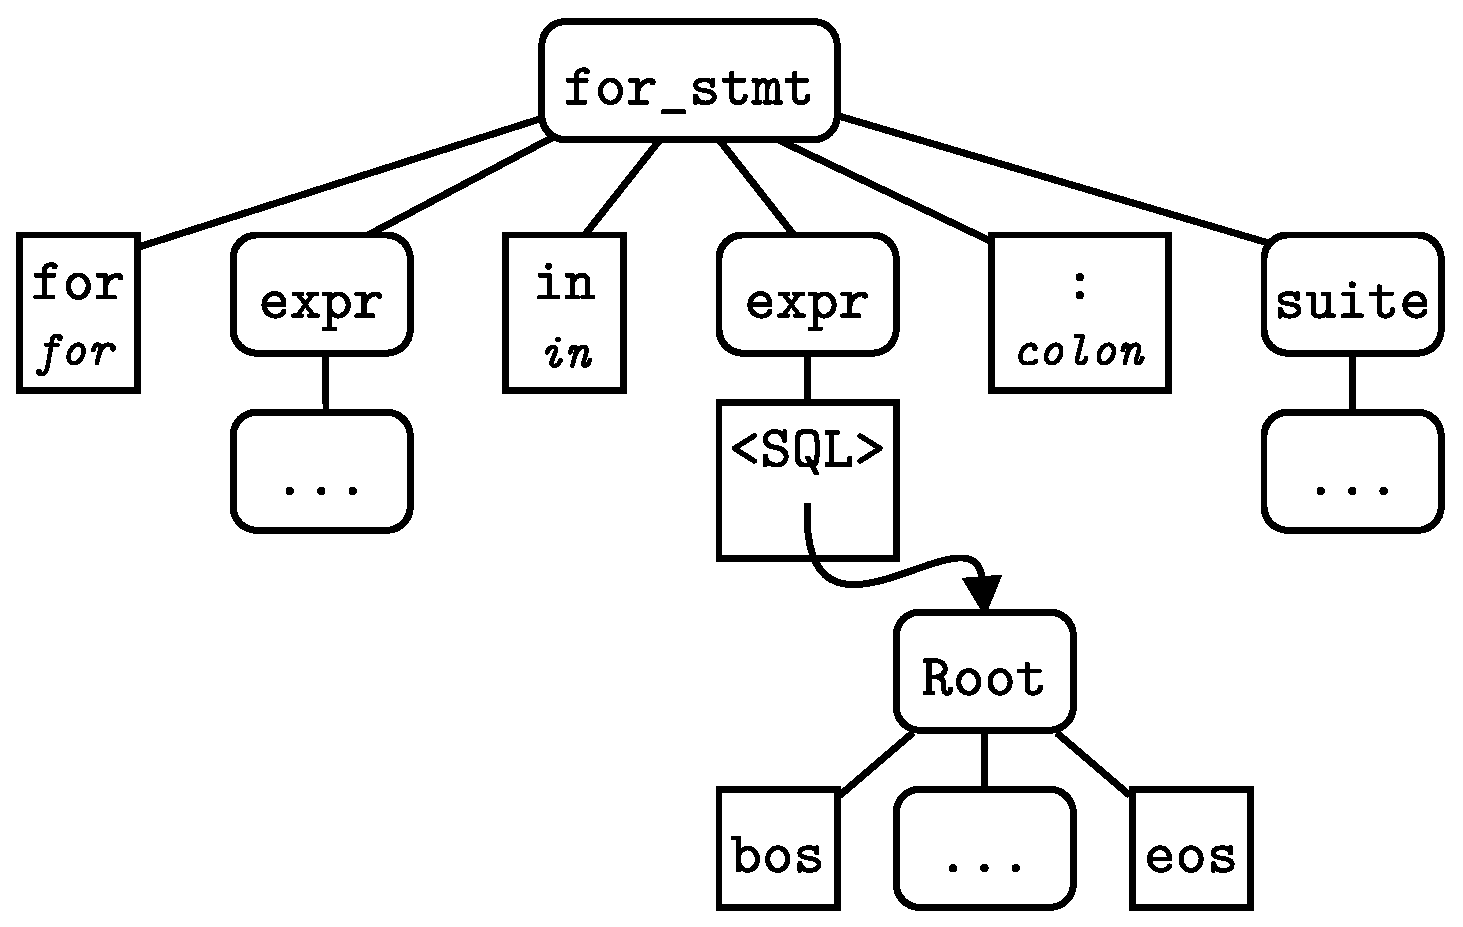
\includegraphics[width=0.35\textwidth]{images/lboxtree}
\caption{An elided example of an SQL language box nested within an outer Python
language box. From the perspective of the incremental parser, the tree stops
at the SQL token. However, we can
clearly see in the above figure that the SQL language box has its own parse
tree, which thus forms part of the wider \inputtree.}
\label{fig:lboxtree}
\end{center}
\end{figure}

Language boxes need to be inserted manually by the user. Though the user may
choose to insert a language box at any place in the program, the validity of
that insertion is restricted by the grammar of the composition. For example,
Figure \ref{fig:langmenu} shows the composition of HTML, Python, and SQL.  The
HTML grammar has been modified to allow Python language boxes to be inserted
anywhere between HTML tags, while the Python grammar has been altered to allow
SQL language boxes wherever Python expressions are valid.  In the example, the
user has already inserted a Python language box into HTML and is about to
insert an SQL language box after the `\texttt{print}' (while arbitrary language
boxes can be inserted, the editor highlights those that are valid in the
current context). If a language box is put into a place where it isn't valid it
will be highlighted as a syntax error. Note that this does not affect the
user's ability to edit the text inside or outside the box, and the editing
experience retains the feel of a normal text editor.

\begin{figure}[t]
\begin{center}
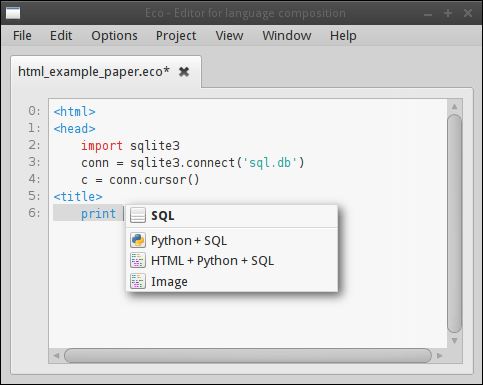
\includegraphics[width=0.48\textwidth]{images/dropdown.png}
\caption{Inserting a language box opens up a menu of the languages that \eco
knows about. Languages which \eco knows are valid in the current context are
highlighted in bold to help guide the user.}
\label{fig:langmenu}
\end{center}
\end{figure}

Typing inside the Python+SQL language box makes it visibly grow on screen to
encompass its contents. Language boxes can be thought of
as being similar to the quoting mechanism in traditional text-based approaches
which use brackets such as $\llbracket~\rrbracket$; unlike text-based brackets,
language boxes can never conflict with the text contained within them. Users can
leave a language box by clicking outside it or using the cursor keys.
Within the parse tree, the
language box is represented by a token whose type describes its language and whose
value is irrelevant to the incremental parser. As this may suggest, conceptually the top-level
language of the file is a language box itself. Each language
box has its own editor, which in this example means each has an incremental
parser.

At the end of the editing process, assuming that the user has a file with no syntax
errors, they will be left with a parse tree with multiple nested language boxes inside
it. In other words, the user will have entered a
composed program with no restrictions on where language boxes can be placed; with no
requirement to pick a bracketing mechanism which may conflict with nested
languages; with no potential for ambiguity; and without sacrificing the ability
to edit arbitrary portions of text (even those which happen to span multiple
branches of a parse tree, or even those which span different language boxes).

\section{Using errors to detect language boxes}
\label{sec_finding_lbox_candidates}
% only on error
% glr style: check on every shift if a box is valid: subsection "Improving
% detection"

In order to insert language boxes automatically we need to be able to determine
where one language ends and another begins. However, since languages may share
a similar syntax this is sometimes even for an experienced programmar an
impossible task. The challenge is thus not to find a perfect solution, but to
find a heuristic good enough to identify as many opportunities for the
automatic insertion of language boxes as possible. Such a heuristic has two
major requirements: it needs to be fast enough to not interfer during editing;
and, more importantly, it must keep the insertion of wrong language boxes to a
mininum, as to not force the user to perform unexpected manual work to revert
the heuristic's mistakes.

Embedding one language into another typically results in a parse error, unless
the embedded input is completely valid in the outer language. Of course, not
every error means that a user intended to insert a language box, and not every
language box a user wants to insert is guaranteed to produce a parsing error.
However, since most languages have a different enough syntax, and searching for
automatic language boxes on every keypress would implicate performance, parse
errors serve as a a good initial heuristic. Figure \ref{fig_heuristic_example}
shows two examples where the embedding of a language into another results in
parse errors which could be used to automatically insert language boxes.

\begin{figure}
    \begin{subfigure}{0.4\textwidth}
    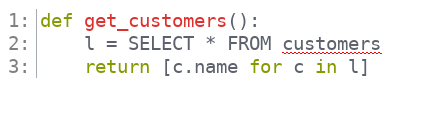
\includegraphics[width=1\textwidth]{images/heuristic1.png}
    \caption{Python and SQL}
  \end{subfigure}
  \begin{subfigure}{0.4\textwidth}
    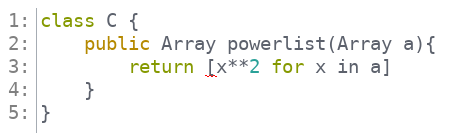
\includegraphics[width=1\textwidth]{images/heuristic2.png}
    \caption{Java and Python}
  \end{subfigure}
\caption{Two examples showing the attempted composition of languages without the
use of a language box. Both compositions result in an error, which can be used
to search the surrounding area for potential language box locations. \textbf{a)}
Here we have to search backwards to `\texttt{SELECT}' at which location the
insertion of an SQL box is possible. \textbf{b)} Here a box can be inserted
immediately at the location of the error.}
\label{fig_heuristic_example}
\end{figure}

When a parse error occurs during parsing, it is analysed immediately. This has
the advantage that we have additional information available (e.g.~the parse
stack) to help us decide whether the insertion of a box is a valid choice.
The basic idea is to analyse the area surrounding the error to find language
box candidates whose insertion remove the error by making the input
syntactically valid. The main challenge is therefore in finding suitable
candidates.

We propose three different heuristics for finding suitable candidates. Each heuristic
starts by searching backwards from the error to find locations where a
language box would be valid. At each location, for each language in the composition,
it then tries to match as much text as possible. If consumed text is valid in one
of the languages, a candidate is produced. Each language can produce multiple
candidates by consuming more text, even if a candidate for that language has
already been found. Afterwards, each candidate language box is virtually
applied to the user's input (replacing the consumed text). If it introduces
extra errors or does not fix the initial parsing error, the candidate is
discarded. If at the end no candidates are found, the error
remains, as normal; if one candidate is found, we automatically insert the
appropriate language box; and if multiple candidates are found, we ask the user
for help.
Listing \ref{lst_find_candidates} shows the heuristics for finding suitable
candidates.
For performance reasons we cannot simply scan the entire input preceding the error,
so each heuristic uses a different approach to reduce the amount of locations that
need to be tested. Neither approach is optimal, since skipping the majority of locations
leads to missed opportunities. However, in conjunction, the heuristics detect a sufficient
number of locations to make automatic language boxes viable.

\begin{figure*}[t]
\begin{minipage}{0.333\textwidth}
\begin{lstdefault}
def find_candidates_stack(error):
  valid_boxes = []
  for lang in <!\textit{composition}!>:
    cut = len(stack)
    while cut >= 0:
      if <!\textit{lbox of lang can be shifted at cut}!>:
        for e in consume_text(stack[cut], lang):
          c = (lang, cut, r)
          if confirm_candidate(c) and \
              fixes_error(c, error):
            valid_boxes.append(c)
      cut -= 1
  return valid_boxes
\end{lstdefault}
\end{minipage}
\begin{minipage}{0.333\textwidth}
\begin{lstdefault}
def find_candidates_history(error):
  valid_boxes = []
  parent = error.parent
  for lang in <!\textit{composition}!>:
    while parent is not None and parent.left:
      if <!\textit{lbox of lang can be shifted after parent.left}!>:
        for e in consume_text(parent.left, lang):
          c = (lang, parent.left, r)
          if confirm_candidate(c) and \
              fixes_error(c, error):
            valid_boxes.append(c)
      parent = parent.parent
  return valid_boxes
\end{lstdefault}
\end{minipage}
\begin{minipage}{0.333\textwidth}
\begin{lstdefault}
def find_candidates_line(error):
  valid_boxes = []
  term = error
  for lang in <!\textit{composition}!>:
    while True:
      if <!\textit{lbox of lang can be shifted after term}!>:
        for e in consume_text(start, lang):
          c = (lang, parent.left, r)
          if confirm_candidate(c) and \
              fixes_error(c, error):
            valid_boxes.append(c)
      if <!\textit{term is newline or BOS}!>:
        break
      term = term.previous_terminal()
  return valid_boxes
\end{lstdefault}
\end{minipage}
\caption{
\lukas{This needs some more work, e.g.~the body of the heuristics is the same and
could be moved to its own function. There is also the question if we need to show
an algorithm at all or if we can abstract this more.}
Each heuristic starts by iterating over all languages $l$ that are part
of the current composition. For each language $l$, it scans the text
before the error to find valid locations where a language box of $l$ can be
inserted. The approach used to scan the preceding text depends on the heuristic.
The stack-based heuristic uses the positions on the current parse stack; the
history-based heuristic traverses the ancestors of the error node in the previous
parse tree; the line-based heursitic scans the terminals preceding the error up to the
beginning of the line.
For each of
those locations the heuristic then tries to consume the following input, using $l$'s lexer and
parser, producing a candidate whenever the consumed text is a valid program in
$l$; \texttt{consume\_text} stops when it can't consume any more input, because either the remaining
input is invalid in $l$, or there is no more text to consume. Afterwards, the heuristic needs to
confirm that the produced candidates fix the previous error and
don't introduce any new ones.
Candidates are returned in the order they are found: the closer to the error and
the shorter they are, the higher they are in the list.}
\label{lst_find_candidates}
\end{figure*}

Despite best efforts,
we will encounter cases where an inserted language boxes is not what the user
intended. The user thus may undo an inserted language box anytime using the,
for editors typical, \keys{Ctrl+Z} key combination. Automatically inserted
language boxes are initially marked as \emph{loose} boxes, which means they may
be automatically removed again or resized to encompass less or more code. The
box remains loose as long as the cursor remains inside it, but as soon as the
user manually moves the cursor out of the box, it becomes \emph{fixed}\lukas{better: locked?} and stays this
way. However, the user may manually mark boxes as loose or fixed as they wish,
via the editor's submenu\lukas{Not yet implemented in Eco}.

\subsection{Finding candidates}

As an example, let's consider a composition of Java and Python, where Python
functions are allowed wherever Java functions are valid. For this we embed into
Java a subset of the Python grammar, accepting only Python functions, which we
call \texttt{pyfuncdef}\footnote{This grammar can be constructed from the
Python grammar (shown in Appendix \ref{app_python_grm}) by changing the start
rule to \texttt{funcdef}.}. We now assume the user wrote the following program:

% Normal example
\begin{lstdefault}[language=Java]
  class Example {
      def x():
  }
\end{lstdefault}
\vspace{1em}

This program currently has a parsing error at \qtt{:}\footnote{The parser
expected an opening bracket here, as Java parses \qtt{def x()} as a function
definition \qtt{x} of the type \qtt{def} which needs to be followed by opening
and closing brackets.}. We now try to find a valid location on the parse stack,
where a \texttt{pyfuncdef} language box can be inserted. Such a location is just
before \qtt{def}.
In the next step we try to find candidates by consuming text, starting at
\qtt{def}.  The language \texttt{pyfuncdef} can consume everything up to, but
excluding \qtt{\}}, which causes a parse error and thus cannot be consumed. The
only consumed text up to that point is \qtt{def x():}, which is not a valid
program in \texttt{pyfuncdef}, and so no candidate is produced as a result.

Assume now that the user inserts \qtt{pass} into the above program, resulting in:

\begin{minipage}{\linewidth}
\begin{lstdefault}[language=Java]
  class Example {
      def x():
          pass
  }
\end{lstdefault}
\end{minipage}
\vspace{1em}

While the error remains at \qtt{:}, more text can be consumed this time. Again,
we use the language \texttt{pyfuncdef} to consume text starting from \qtt{def}.
Upon consuming \qtt{pass}, a valid Python function has been found and a
candidate is created. We continue consuming text, to find further candidates.
However, as before, we stop upon reaching \qtt{\}} which is not valid in
\texttt{pyfuncdef}. Having found a candidate, we now need to check if it fixes
the error and doesn't introduce any other errors immediately following the box,
when it's applied to the users input. We replace the consumed text with a
language box of \texttt{pyfuncdef} and attempt a parse in the outer language,
Java, starting at the location of the language box.
As soon as we successfully parsed \qtt{\}} we can stop,
confirming that the insertion of the candidate doesn't introduce
any new errors (Section \ref{sec:parse_after_lbox} discusses why it is
sufficient to stop parsing after \qtt{\}} and why we don't have to parse the
entire program to determine if the candidate is valid). Finally, we check if
the original error has been eliminated, which is the case here, as the error
node \qtt{:} was included in the candidate language box. The candidate is thus
valid and can be automatically inserted into the program.

\subsection{Confirming candidates}
\label{sec:parse_after_lbox}

In order to confirm if a candidate is valid, we need to
check that it does not introduce new errors when it is inserted into the parse
tree, and also that is fixes the initial parsing error. In order to determine if a
candidate doesn't introduce new errors, we can simply check if the first
non-whitespace token that follows it can be shifted.  The reasons for this are
twofold. Firstly, we don't want to parse too far past the language box for
performance reasons, and because this could lead to candidates being falsely
rejected (see Figure \ref{fig_autoboxerrorafterinsert} for an example).
Secondly, whitespace tokens, which most programming languages use, have the
property, that they can almost always be shifted after another token. This
means that a whitespace token following a language box candidate would always
confirm the candidate, even if the insertion of the box would cause an error
immediately after that whitespace. This can sometimes lead to invalid
candidates being accepted (see Figure \ref{fig_autobox_nonwhitespace} for an
example).

\begin{figure}
\begin{center}
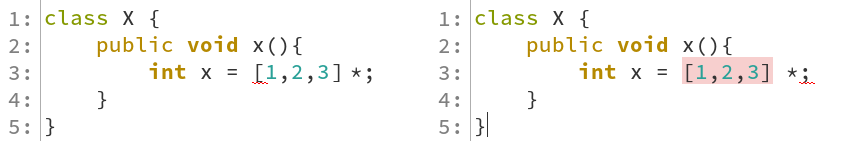
\includegraphics[width=0.50\textwidth]{images/autoboxerrorafterinsert.png}
\end{center}
\caption{An example showing why parsing further than necessary to confirm
a language box candidate, can lead to the candidate being falsely rejected.
The example shows a composition of Java and Python, that allows Python
expressions wherever Java expressions are valid. The user inserted a Python list
into the program (left), which produced a language box candidate (right). To validate
the candidate we insert it into the program and parse it. However, after parsing \qtt{*},
an error occurs which would invalidate the constraint that an automatic
language box shall not introduce new errors, and thus reject the candidate,
despite this being an otherwise valid insertion.}
\label{fig_autoboxerrorafterinsert}
\end{figure}

\begin{figure}
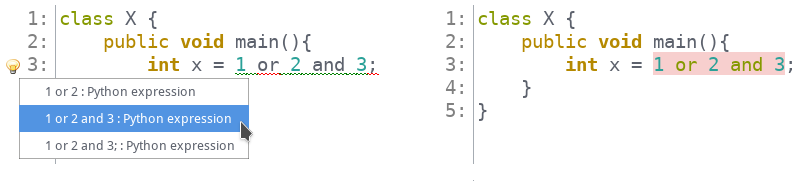
\includegraphics[width=0.5\textwidth]{images/autobox_nonwhitespace.png}
\vspace{0.3em}
\caption{An example showing how using only non-whitespace tokens to confirm language
box candidates gives better results. The example uses a composition of Java
and Python, which allows Python expressions in place of Java expressions. The
user just pasted the Python code \qtt{1 or 2 and 3} into the assignment, in
between \qtt{=} and \qtt{;}. \textbf{a)} If we use any first token to confirm
candidates, we get three results. The first option, \qtt{1 or 2},
is a valid candidate, because the following token is whitespace, which can
be shifted, confirming the candidate; however the following
\qtt{and} then causes an error. The same is true for the third option, \qtt{1 or 2 and 3;}, which is
followed by a newline, which confirms this candidate, even though the \qtt{\}} then
errors because the semicolon of the assignment was included in the Python
language box. \textbf{b)} When using the first non-whitespace token for candidate
confirmation, we reduce the three options to one, which can then be automatically
inserted.}
\begin{picture}(0,0)
  \small
  \put(-110,225){\textbf{(a)} Using first token}
  \put(-20,225){\textbf{(b)} Using first non-whitespace token}
\end{picture}
\label{fig_autobox_nonwhitespace}
\end{figure}

% Multiple choice example
\subsection{Handling multiple solutions per language}

While many compositions only have one valid outcome, sometimes there are
multiple options for the insertion of a language box. This can be either that
there are multiple languages that can be inserted, or that there are multiple
variants of consumed text for a single language.  An example for the latter is
shown in the following composition of PHP and Python, which allows any Python
box wherever a PHP expression is valid.

\begin{center}
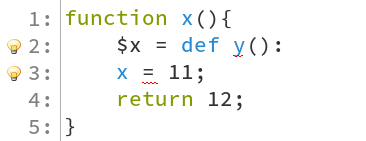
\includegraphics[width=0.25\textwidth]{images/autoboxmultioption.png}
\end{center}

In the example there are two options to fix the error at \qtt{y} in line 2, via
the insertion of a Python box. We can include everything from \qtt{def} up to,
and including \qtt{return 12}, or we can stop after \qtt{x = 11}.  Since both
options are valid and fix the error, we can't automatically pick one.
Instead, we display an indicator that there are multiple solutions available
(in the examples this is shown via a light bulb icon next to the line numbers). From
there the user can choose one of the solutions from a drop-down list. Clicking
on one of the options then automatically inserts a language box and replaces
the relevant code:

\begin{center}
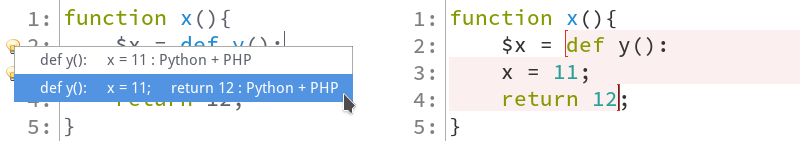
\includegraphics[width=0.50\textwidth]{images/autoboxmultioption2.png}
\end{center}

\subsection{Limiting automatic insertions}
\label{subsec:limitingautoinserts}

Some grammars can be very unrestrictive, allowing almost any text to be valid.
In HTML, for example, any combination of characters that does not contain
\qtt{<} or \qtt{>} is a valid program. Unfortunately, this means that in a
composition with HTML most errors can be solved by simply wrapping them with a
HTML language box, often resulting in something the user didn't intend. For
instance, the following example shows a program written in a composition of
Python that allows SQL and HTML wherever Python expressions are valid:

\begin{center}
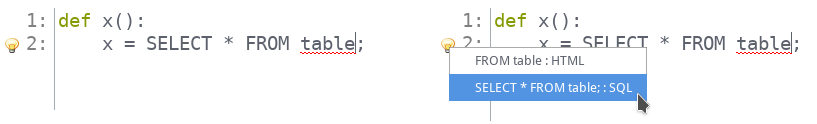
\includegraphics[width=0.5\textwidth]{images/auto_html.png}
\end{center}

We can see that the error at \qtt{table} can be solved by either wrapping
\qtt{SELECT * FROM table} into a SQL language box, or by just wrapping
\qtt{FROM table} into a HTML language box. While a human can easily guess
that the user meant to insert a SQL box here, this scenario is impossible for the
algorithm to detect. To remedy this the creator of the language composition can add hints that
limit the insertion of some language boxes in such cases.   There are two ways in which
a language author can add limitations to a composition: 1) They can define
the symbols that an automatically inserted language box must start with 2)
or they can exclude specific symbols that must not appear at the beginning of a
language box. For example, to solve the above problem, they user could define
that a HTML box should only be inserted if the box starts with a HTML tag,
e.g.~\qtt{<img}.

Of course, another valid solution is to simply define a more
fine-grained composition. For example, instead of creating a Python/HTML
composition that allows all HTML to be valid wherever Python expressions are
valid, the composition could be restricted to only allow HTML-tags
(e.g.~\qtt{<img}, \qtt{<html}, etc) by embedding only a subset of the HTML
grammar. However, this depends on the make-up of the grammar, and may not
always be possible it doesn't separate rules on such a fine-grained
level.

\subsection{Automatically removing boxes}
\label{subsec_autoremoval}

Despite the solutions described in \ref{subsec:limitingautoinserts} there
will always be some remaining cases where automatically inserted language boxes do not match the
user's intentions. While the user can always undo a wrong insertion,
we do not want to burden them with the task of repeatedly
cleaning up the algorithm's mistakes. The following composition of Python and
SQL, though admittedly a rather unlikely scenario, exemplifies the problem:

\begin{lstdefault}[language=Python]
  def x():
    SELECT = 1
    FROM = 2
    table = 3
    x = SELECT * FROM table
\end{lstdefault}
\vspace{1em}

After typing in this program, an SQL language box will have been automatically
inserted, replacing the text \qtt{SELECT * FROM table}. From a syntax
perspective, this was a valid decision. However, we can see from the variable
declarations that the user's intention was to multiply the three poorly named
variables and simply forgot a \qtt{*} between \qtt{FROM} and \qtt{table}.
Instead of requiring the user to manually undo the insertion, \eco can
automatically remove inserted language boxes again once more information has
become available.  In this example, once the user inserts the missing \qtt{*}
between \qtt{FROM} and \qtt{table}, the SQL language box becomes invalid. This
gives us a good clue that the language box was inserted accidentally and needs
to be removed; with the restriction, that its entire content must be valid in
the outer language.
However, sometimes an automatically inserted language box can become valid in
both the inner as well as the outer language, after the user made additional
changes.  In those cases \eco prioritises the outer language and removes the
box, but only if the boxes contents \emph{and} its surrounding context can be
parsed in the outer language.  The following constraints summarise the above
(an example using these constraints is given in Figure \ref{fig_autoremoval}):
\begin{enumerate}
  \item Only automatically inserted boxes can be automatically removed again.
  \item If the language box content is invalid, it will be removed only if
        its content can be parsed in the outer language.
  \item If the language box's content is valid in both the inner and outer
    language, it will be removed only if its removal doesn't introduce new errors (i.e.~if its contents \emph{and} the first non-whitespace token following it
    can be parsed).
\end{enumerate}

Using these constraints for the example from before, the inserted box would be
removed as soon as the user inserts a \qtt{*} between \qtt{FROM} and
\qtt{table}; however, it stays if more SQL code is added even it that makes the
SQL code temporarily invalid. Note that language boxes that were inserted by the
user, via choosing one of the suggested candidates, count as manual insertions
and won't be automatically removed, even if they become invalid.


\begin{figure}
\begin{center}
\vspace{0.8em}
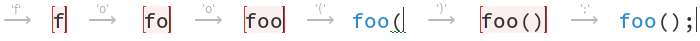
\includegraphics[width=0.45\textwidth]{images/autoremove_foo.png}
\vspace{-0.8em}
\end{center}
\caption{An example showing the constraints for automatic language box removal in practice.
The example uses a composition of PHP and Python where Python expressions are valid at
PHP's top-level.
We can see that as the user types, language boxes are getting automatically
inserted and removed depending on their content. At the beginning the user types
\qtt{f}, which is not valid in PHP and thus gets replaced by a Python
language box, making the program valid again. The box stays until the user
inserts \qtt{(} which makes the Python language box invalid, and since all of
its content can be parsed in the outer language, the box is removed.
As soon as the user inserts the closing bracket \qtt{)}, a Python box is
inserted again to fix the PHP parsing error caused by a missing semicolon. When the
user eventually inserts the missing semicolon the contents of the language box
are valid in both PHP and Python. However, since the box can be removed
without introducing an error, we prioritise the outer
language, and remove it again.}
\label{fig_autoremoval}
\end{figure}

%After a language box has been inserted it stays in a "to be determined"
%mode. When the user moves the cursor outside the box, the box is finalised. Until then,
%any changes inside the box have to be validated and can lead to the box being destroyed again.
%E.g. changing \qtt{x = SELECT * FROM table;} to \qtt{x = SELECT * FROM} will remove the box again
%as the content is valid Python now and not valid SQL anymore.

\subsection{Resizing language boxes}

Language boxes may automatically resize if this allows both the language box as
well as the outer program to parse correctly. A language box may shrink, if it
contains an error which can be resolved by moving contents into the outer
language. It may expand if tokens following it can be included in the box,
especially if those tokens are syntactically incorrect in the outer language
\lukas{We have a design choice here: Should a language box always encompass the
maximum amount of code, or should it only grow if it can remove errors in the
outer language doing so?}

\section{Limitations}
\label{sec_lbox_limitations}

This section highlights the limitations of the heuristic used, by giving some
examples of ambiguities that cannot be resolved with automatic language boxes,
resulting either in unwanted or no language boxes being inserted.

\subsection{No detection}

One example, where error based detection of automatic language boxes doesn't
work, is when the outer language can match everything in the inner language.
For example, HTML can match arbitrary text between tags. This makes
compositions, where other languages are embedded into HTML, impossible to
detect automatically. The following code example shows this:

\begin{lstdefault}[language=html]
<html>
import sqlite
sqlite.connect("test.db")
</html>
\end{lstdefault}
\vspace{1em}

Since HTML allows any text in between its tags, the insertion does not cause an
error, and thus the \ald is never called to detect automatic language boxes.
However, even to a human it is unclear if the user meant to insert a Python
box, or simply wanted to print out the code in HTML. Although, a non-error
based heuristic for finding language box candidates could at least show the
user that a language box would be possible.  A naive example for such a
heuristic could try to match language boxes at each terminal location. However,
such a solution would be much slower than the error based approach.

\subsection{Wrong detection}

Another problem is when the insertion of an automatic language box extends into
parts of the outer language, even if those parts weren't meant to be included
inside of the box. For example, this can occur when composing Java and Python,
allowing Java functions to be replaced with Python functions, as shown below:

\begin{center}
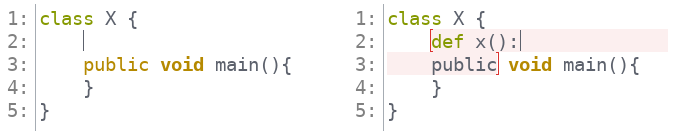
\includegraphics[width=0.50\textwidth]{images/autobox_limitjavapy.png}
\end{center}

The user attempted to insert a Python function above the Java function.
However, as the user was typing, a box was automatically inserted which
extended into the Java function, and used the keyword \qtt{public} as the body
of the Python function.  This is valid, since the keyword is optional in Java,
so the insertion of that box does not create any errors, even though it is
clearly not what the user intended.
This problem can be circumvented by restricting the tokens that are allowed to
be parsed to only the most recent ones. Since the user is most likely to type
from top to bottom, we can disallow any tokens to be included in the language
box that are older than the starting token. Since the \qtt{public} token was
typed before the user started typing the Python code, it won't be included in
the box, thus avoiding this issue\lukas{This also affects the last example in
Section 3.3}. The downside to this is, however, that it won't be possible for
the user to type language boxes out-of-order.  For example, they can't start
typing the body of a Python function and add the method header afterwards, as
then the body will be older than the header.

\subsection{Grammar limitations}

Sometimes the structure of a grammar can be responsible for the failure to
generate automatic language boxes. For example, let's consider a composition of
PHP and Python, that allows Python expressions wherever PHP expressions are
valid. The user then edits the composition as follows:

\begin{center}
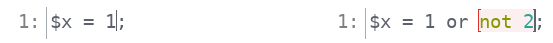
\includegraphics[width=0.45\textwidth]{images/autobox_limitphpgrammar.png}
\end{center}

The user might reasonably expect to have a second option here, which would
allow the content \qtt{1 or not 2} to be wrapped into a Python language box.
The algorithm, however, couldn't detect this and instead only found a single
candidate, \qtt{not 2}, which was automatically inserted.  The problem lies
within the PHP grammar, which also has a keyword \qtt{or}, and how the location
for language box candidates are calculated. As described earlier in this
chapter, we use a technique similar to error recovery, that rewinds the parse
stack to find a position on the stack, where the language can be inserted.
However, the way the PHP grammar is structured and thus parses the above input,
makes it impossible to find a location on the stack that allows \qtt{1 or not
2} to be wrapped into a language box, as Figure \ref{fig_auto_phplimit} shows.

\begin{figure}
\begin{center}
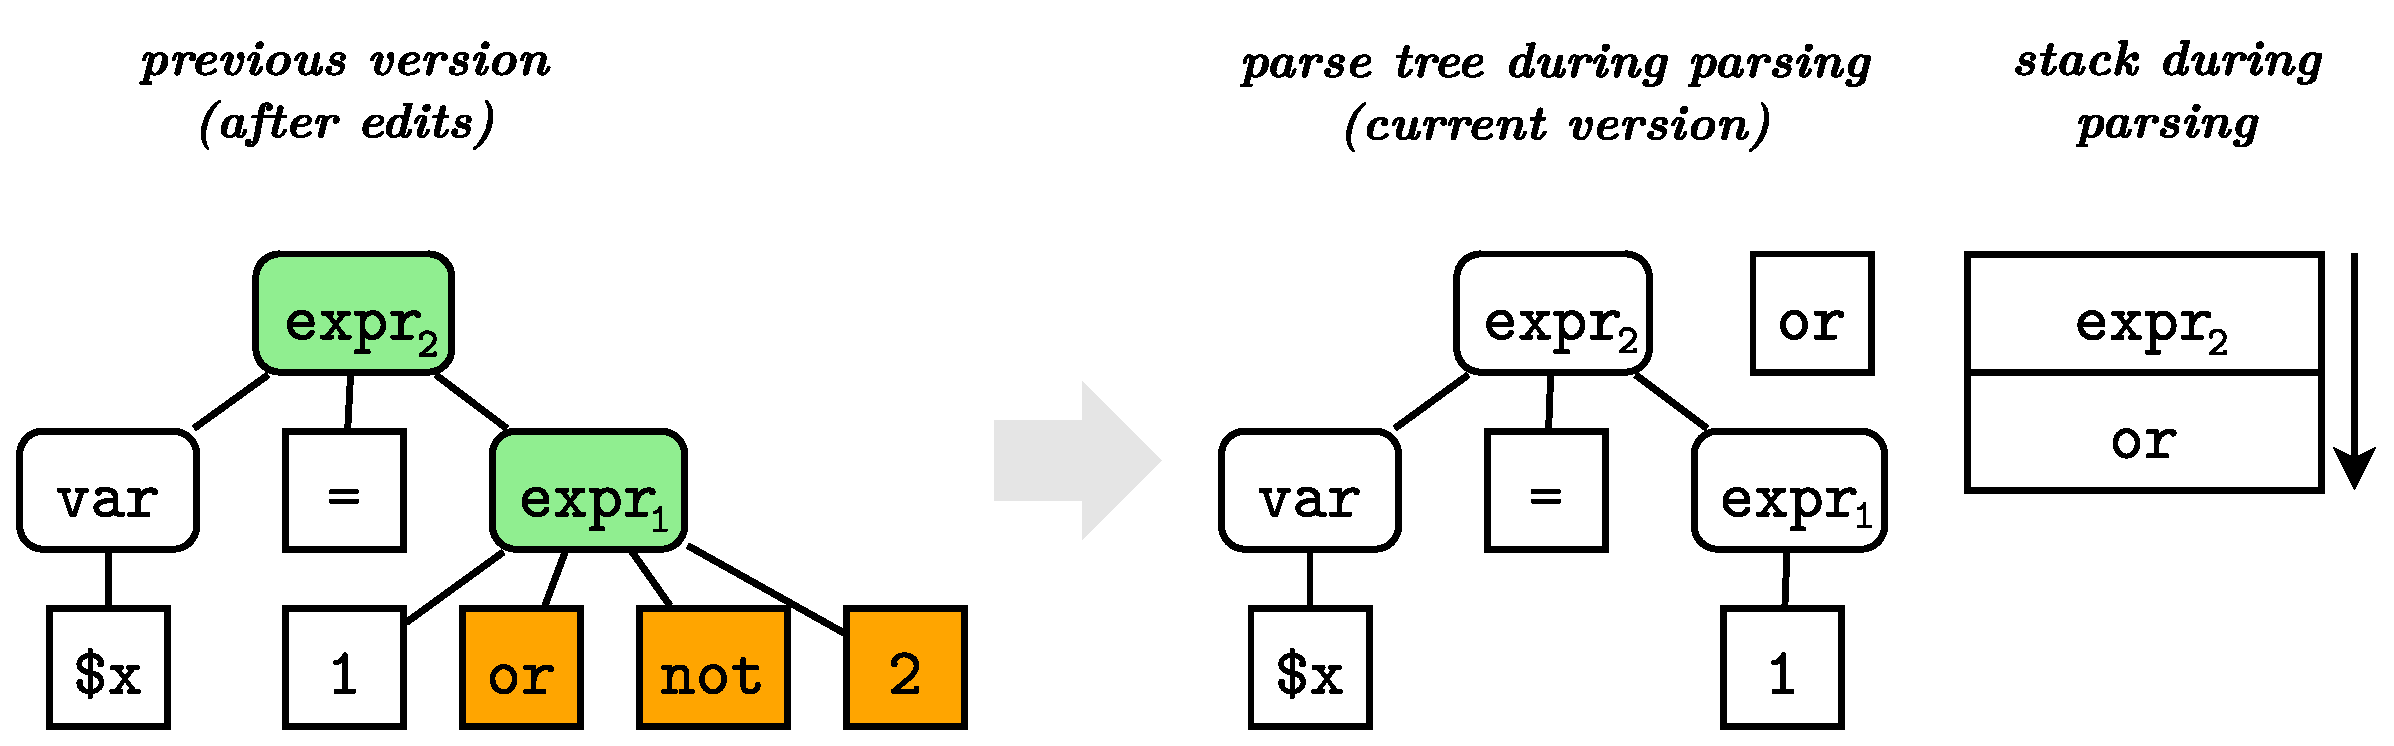
\includegraphics[width=0.49\textwidth]{images/limitation_php}
\end{center}
\caption{An example showing how sometimes the grammar of a language can
keep the automatic language box detection from finding appropriate candidates.
Shown on the left is the elided parse tree after the user edited the PHP expression
\qtt{\$x = 1;} by inserting the Python code \qtt{or not 2}. However, we
can see on the right, that by the time the error occurs, PHP has already reduced \qtt{\$x = 1} to \texttt{expr\textsubscript{2}}, and shifted
\texttt{or} onto the stack. The only valid locations for a language
box we can thus find are before \texttt{expr\textsubscript{2}} and \qtt{or}. In particular,
we cannot find the location before \qtt{1} which would allow us to wrap the entire expression
into a box.}
\label{fig_auto_phplimit}
\end{figure}

Other compositions suffer from the same issue:
\begin{itemize}
    \item[JavaLua] `\verb|int x = 1, 2|', can't wrap `\verb|1, 2|' in a Lua
        language box, since Java has already reduced parts of the parse tree
        after seeing the `\texttt{,}', so that neither heuristic can reach the
        beginning of the expression.
    \item[JavaSQL] `\verb|int x = BEGIN; SELECT a FROM t;|'. Since `\texttt{BEGIN;}` is a
        valid Java expression, it has already been reduced to a subtree which
        can't be reached from the error that occurs in `\texttt{FROM}'.
    \item[LuaJava] `\verb|x = new int[1]|'. Error occurs after the Java expr, at
        which point it has already been reduced in Lua.
    \item[LuaSQL] `\verb|local x = SELECT a, b FROM t1;|'. After parsing
        `\texttt{,}', the parse tree is reduced in a way that makes reaching the
        beginning of the expression impossible for the heuristics.
    \item[LuaSQL] `\verb|local x = SELECT a.b FROM t1;]|'. Same as the above but
        with `\texttt{.}' instead of `\texttt{,}'.
\end{itemize}

\subsection{Problems with comments}

Sometimes comments can be the reason for a failed insertion. For example, when
composing Lua and Java, a possible composed program may look like this:

\begin{lstdefault}[language={[5.2]Lua}]
function decrease(x)
    y = --x
    return y
end
\end{lstdefault}

where `\verb|--x|' is meant to be a Java expression. However, since `\texttt{--}'
in Lua is a comment, the error happens later in `\texttt{return}', making it
impossible for the heuristic to find the beginning of the expression.
Similarly, when composing Java and Lua while using Lua's floor division, e.g.~
`\verb|int x = 3//4 + 1;|', no language box is inserted, as `\texttt{//}' is interpreted
as a Java comment, which means the error occurs at a location which makes it impossible
for the heuristic to find the beginning of the expression.

Another problem with comments appears in compositions of PHP and SQL:

\begin{lstdefault}[language=PHP]
$x = SELECT a FROM t1 -- comment;
$y = 2;
\end{lstdefault}

At first, when typing the SQL statement, as language box is correctly inserted
around \verb|SELECT a FROM t1|. However, after typing the first \texttt{-}
inside the language box, the box is shrunken, moving the \texttt{-} to the
outside. One would assume that the box gets expanded again as soon as we
continue typing the comment. However, when testing if the box can be expanded,
the lexer for SQLite lexes the entire comment to the end of the line, including
the semicolon finishing the PHP statement. Without this semicolon, PHP cannot
parse successfully, breaking the condition for the expansion, which is thus
aborted. The same problem can appear in other compositions where semicolons are
used to end a statement, e.g.~Java.

\subsection{Problems with strings}

Some languages, like PHP, allow newlines within strings. Embedding such a
language inside another language can thus sometimes require the entire file to
be lexed during automatic language box detection. For example when typing the
PHP expression \texttt{\$x = 'a'} into Java, this will cause the entire
remaining Java program to be lexed as long as the single quote has not been
closed. However, since the lexing only happens virtually and is not applied to
the input (unless this result in the insertion of a new language box), this
does not affect the parse tree of the outer language. And since lexing is
generally quite fast, the performance impact will also be insignificant.

\section{Recognisers}
\label{sec:impl_defaultrec}

This section describes in more detail how language box candidates are
constructed and how we can improve performance by not using a full incremental
parser to find language box candidates, but instead using a simple batch
recogniser. A recogniser is a parser that doesn't execute any actions or
generates a parse tree, but rather only validates the input. This section also
shows how a recogniser can be used to decide whether or not a language box can
be removed again.

Section \ref{sec_finding_lbox_candidates} described, how in order to find
language box candidates, we try to consume as much text surrounding the error
node as possible, generating a candidate every time the surrounding text is
valid in the language of the box. Since we are only interested in the text that
can be parsed and don't need to generate a parse tree from it, a simple batch
recogniser is a good alternative to a full parser, as it improves performance
and reduces memory usage.  An important restriction is that the recogniser must
lex and parse input from the parse tree without actually altering the parse
tree or any nodes within it.  A recogniser in the \ald takes as input a node
from which it starts parsing, and returns all valid substrings from that input,
until either a parsing error occurs, or there is no more input left to parse.
Substrings are returned in form of their end node in the original parse tree.
The substring can then be derived by reading all tokens between the start and
end node.  The algorithm is shown in Listing \ref{lst_consume_text}.

\begin{figure}
\begin{lstdefault}[]
def consume_text(node, lang):
  lexer = <!\textit{lexer for lang starting at node}!>
  parser = <!\textit{parser for lang}!>
  results = []
  token = lexer.next_token()
  while token is not None:
    if parser.parse(token):
      if <!\textit{parser can accept current input}!>:
        results.append(lexer.last_node)
    else: # parse error
      break
    token = lexer.next_token()
  return results
\end{lstdefault}
\caption{An algorithm for consuming text and returning valid
substrings for the creation of language candidates. We first create a lexer that
produces tokens in language \texttt{lang}, starting at \texttt{node} (line 2).
We also create a parser for \texttt{lang} (line 3) which is used to parse input (line 7) and test if the
input parsed so far can be accepted (line 8); the latter can be achieved by simply pretending
that the next token is the end-of-file token, and test if the
parser reaches an accept state. We then consume as much text as we can,
producing tokens and parsing them (line 6--12), until no more text can be
consumed, either due to an error (line 10), or because we've reached the end of
the input. Each time a token was successfully parsed, we test if the input parsed so far is
valid (line 8), and if so, store the last node from the original parse tree that the lexer
processed (line 9). This node is later used to derive the substring from which the
language box is created.}
\label{lst_consume_text}
\end{figure}

\subsection{Recognising Python}
\label{sec:impl_wsrec}

In order to produce language box candidates for whitespace-sensitive languages
like Python, we need to be able to create indentation tokens during the
consumption of input. To do
this, we implement a separate recogniser for Python which uses a wrapper around the lexer that inspects
the tokens that the lexer produces and, when appropriate, returns indentation
tokens instead. While the Python recogniser inherits most of the behaviour of
the default recogniser, it also needs to keep track of the indentation levels. Listing
\ref{lst_next_token_indent} shows how the recogniser wraps around the lexer and
produces indentation tokens whenever they are needed.

\begin{figure}
\begin{lstdefault}[basicstyle=\linespread{1.0}\footnotesize\ttfamily]
def next_token(todo, indent):
  if todo:
    return todo.pop(0) # return first element
  token = lex.next_token()
  if token is <!\textit{newline}!>:
    prevl = <!\textit{previous line}!>
    currl = <!\textit{current line}!>
    if prevl is not empty:
      todo.append(<!\textit{NEWLINE}!>)
    if currl is not empty:
      if prevl.ws < currl.ws:
        indent.append(currl.ws)
        todo.append(<!\textit{INDENT}!>)
      elif prevl.ws > currl.ws:
        ws = indent.pop()
        while ws > currl.ws:
          todo.append(<!\textit{DEDENT}!>)
          ws = indent.pop()
        if ws != currl.ws:
          todo.append(<!\textit{UNBALANCED}!>)
  todo.append(token)
  return todo.pop(0)
\end{lstdefault}
\caption{To support language box detection for Python, we
create a method that wraps around the lexer and produces indentation tokens as
needed by keeping track of the indentation levels. Producing and returning
indentation tokens delays the parsing of tokens which have already been lexed.
In order to not forget to parse those tokens, we use a to-do list (line 3). We
always return the first item of that list. If it is empty, we continue lexing
from the input (line 4). The remaining code is similar to the batch indentation
approach described in Section \ref{subsec_indentation_batch}.
}
\label{lst_next_token_indent}
\end{figure}

\subsection{Incremental Recogniser for auto removal}
\label{sec:impl_removerec}

Section \ref{subsec_autoremoval} described how automatically inserted language
boxes can automatically be removed again, if they become invalid. The condition
for this is that the box's content is valid in the outer language.  In essence,
we need to temporarily remove the language box, paste its content where the box
was before, and then check if the program can still be parsed; of course
without actually altering the parse tree. A recogniser is thus again a good
choice. In order to test if the contents of the box are valid in the outer
language, we first need to initialise the recogniser to the state just before
the language box would be parsed. We can do this incrementally, by only
traversing subtrees that are direct ancestors of the language box. All other
subtrees can be skipped (i.e.~incrementally shifted) similar to the default
incremental parser.

This process is implemented via an additional method \texttt{preparse}, which
incrementally initialises a recogniser's parsing state to the state just before
a given node. Figure \ref{fig_preparse} shows an example of a parse tree, where
we want to test if a language box can be removed, and the algorithm to
initialise the recogniser.
After the recogniser has been initialised, we simply use \texttt{consume\_text}
to parse the content of the language box. If the entirety of the language box
can be successfully parsed in the outer language, the box can be removed.  Of
course, depending on the parsing status of the box, we may also need to parse
at least one non-whitespace token following the former language box.

\begin{figure}
\begin{minipage}{0.45\textwidth}
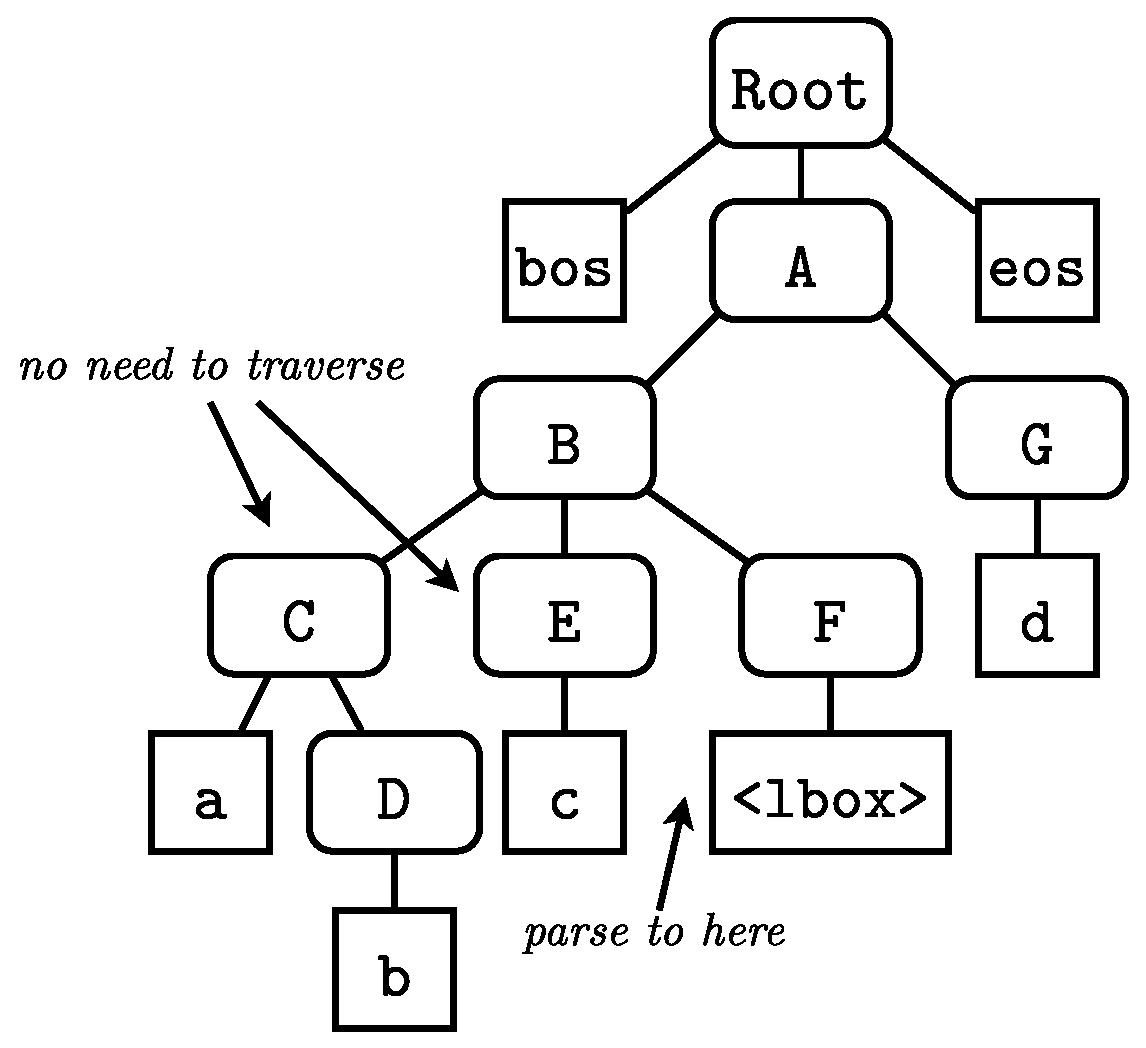
\includegraphics[width=0.9\textwidth]{images/autoremoval}
\end{minipage}
\begin{minipage}{0.5\textwidth}
\begin{lstdefault}[basicstyle=\linespread{1.0}\footnotesize\ttfamily]
def preparse(bos, lbox, parser):
  # "mark" ancestors of lbox
  path_to_lbox = set()
  parent = lbox.parent
  while parent is not <!\textit{Root}!>:
    path_to_lbox.add(parent)
    parent = parent.parent

  # initialise parser
  node = bos
  while node is not lbox:
    if node not in path_to_lbox:
      parser.parse(node)
    else: # traverse node
      if node.children:
        node = node.children[0]
      else:
        node = node.right_neighbour()
\end{lstdefault}
\end{minipage}
\caption{A parse tree with a language box that we want to automatically remove (left)
and the preparse-algorithm (right). In
order to test if the box's content is valid in the outer language, we
initialise a recogniser to the state just before we would parse the language box,
using the recogniser's \texttt{preparse} method. This is done,
by `marking' the ancestors of the language box, as if the language box
contained changes (lines 3--7), and then incrementally parse those subtrees
up to the box (lines 10--18).}
\label{fig_preparse}
\end{figure}

\section{Related Work}
\label{autobox_related_work}


Scannerless parsing~\cite{visser97scannerless, vandenbrand02disambiguation} is well
suited for language composition since it can parse any context-free grammars
which are closed under composition. A notable example of this is
Spoofax~\cite{kats10spoofax}, a language workbench for extending and composing
context-free grammars.
Although scannerless parsing can parse ambiguous programs by creating a parse
forest, it is still necessary to reduce the parse forest into a single
parse tree in order to compile or interpret it. A common way to reduce the parse forest is to
remove all parse trees that are invalid when considering additional information
about the input, such as types~\cite{vinju05typedriven}. Using type information can avoid the
need for separators to disambiguate languages in many cases, however still
requires a set of disambiguation rules, such as preferring identifiers in the
outer language (i.e.~the meta language) over those in the inner language
(i.e.~the object language), or choosing the shortest path if multiple valid
options are available. Unfortunately, not all ambiguities can be solved this
way, making the use of separators still a necessity.

Choosing separators is not trivial, since they can still introduce ambiguities
if the same separator symbol is used for different nonterminals of the embedded
language. This requires \textit{explicit disambiguation}, i.e.~using a
different separator for each embedding with a different nonterminal symbol,
e.g.~\verb|cls{...}cls| for embedding classes and \verb|func{...}func| for
functions~\cite{batory98jts}. Since this can
quickly cause ``syntactic clutter``~\cite[p.~4]{bravenboer05generalized},
an alternative solution is to use type information to automatically disambiguate
embeddings, thus reducing the amount of unique separators that would otherwise
be required~\cite{zook04generating, bravenboer05generalized}.
Unfortunately, since these approaches are dependent on types, they do not work
for dynamically typed languages. Furthermore, heuristics such as picking the
shortest path on multiple valid options can hide options the user cares about
(as shown in Section~\ref{auto_handling_multiple_solutions}).

Despite these improvements, Spoofax's grammar definition SDF,
which allows arbitrary CFGs, can give no guarantees that its grammars are unambiguous,
even more so when they are composed together, since composing two unambiguous grammars can lead to an ambiguous one.
Spoofax thus uses reject grammars, which solve this problem, but
make such grammars context-sensitive~\cite{eijck__lets_accept_rejects}.

Another notable example for language composition is Copper~\cite{wyk07context}
which implements a context-aware scanner to solve ambiguities in language
compositions. The basic idea is that the parser can tell the scanner which
tokens it can parse next and the scanner can only return results from that list.
This means that if two composed languages have similar tokens (e.g.~keywords,
identifiers), the lexer solves ambiguities
by returning the token for the language that it is currently parsing (i.e.~that is currently in context). This allows
Copper to compose languages by extending the host language's grammar rules
with references to rules in the embedded language. However, at the point where
another language can be embedded, i.e.~where the two languages meet, a token
may be valid in both the host as well as the embedded language.
Copper solves this problem
via \texttt{dominates} clauses which are defined within the lexing rules. For example, if an
identifier in the host language clashes with a keyword in the embedded language,
then we can define a clause that says that the keyword dominates the identifier
and needs to be prioritised. Unfortunately, this has the
downside that those tokens cannot be used in the host language at that point,
restricting the host language's expressiveness. This also means that each
composition needs to determine all of those cases and modify grammar and lexer in ways that solve
these ambiguities, making it impossible to create a one-size-fits-all solution for
arbitrary compositions.

\section{Evaluation}

To evaluate the accuracy of automatic language boxes, we ran an experiment,
testing each heuristic on multiple benchmarks. Each benchmark uses a
compositions of two languages, where expressions or functions from one language
can be embedded into the other. The benchmark then first chooses a random file
that parses in the main language. It then picks a random expressions or
function written in the embedded language, and inserts it at a valid location
in the chosen file. All files and expressions/functions were extracted from
real-world programs.

Figure \ref{tbl_valid} shows the total percentage of
acceptable outcomes for each heuristic used broken down by each composition.
Acceptable outcomes are one of the following: a language box gets succesfully
inserted; no language box was inserted since the insertion was already valid in
the outer language; the insertion had multiple options which are presented to
the user.

The results show that while each heuristic has weaknesses, when put together
they result in over 96\% of acceptable outcomes. Weaknesses in the heuristics
are based on the composition. For example, the history-based heuristic only
achieves 67\% of acceptable outcomes when used on the Java+Lua composition. The
reason for this low number can be accounted to the insertion of Lua functions
right after a Java comment.  Since the insertion is attached to the comment
subtree, the history-based heuristic is not able to find a valid location for
the language box by traversing the parse tree.  The line-based heuristic on the
other hand has difficulties with the composition of Java+PHP. The reason for
this is that PHP's function syntax is similar to Java's, e.g.~\texttt{function
x() \{\}} is a valid Java function, where \texttt{function} represents a type.
This leads to many errors only occuring in one of the following lines, which
the line-based heuristic can not deal with. The stack-based heuristic also has
a weakness with the composition of Lua+SQLite. The problem here is related to
the way Lua parses certain inputs. For example, when composing \texttt{x =
SELECT a, b FROM t}, everything up to `\texttt{b}' can be parsed in Lua,
leading to a reduction. This reduction removes \texttt{SELECT} from the stack,
replacing it with a subtree and making it impossible to find a valid location
to insert a language box at.

\begin{figure*}[hbt]
    \begin{tabular}{l  c  c  c  c  c  c  c  c  c  c  c  c  c }
    \toprule
        & \rotatebox{65}{JavaLua} & \rotatebox{65}{JavaPHP} & \rotatebox{65}{JavaSQLite} & \rotatebox{65}{LuaJava} & \rotatebox{65}{LuaPHP} & \rotatebox{65}{LuaSQLite} & \rotatebox{65}{PHPJava} & \rotatebox{65}{PHPLua} & \rotatebox{65}{PHPSQLite} & \rotatebox{65}{SQLiteJava} & \rotatebox{65}{SQLiteLua} & \rotatebox{65}{SQLitePHP} & \rotatebox{65}{Overall} \\
    \midrule
    Corpus size & 950 & 889 & 659 & 295 & 265 & 170 & 557 & 500 & 317 & 282 & 289 & 281 & 5,454 \\
    \midrule
    All & 99.4\% & 94.6\% & 99.7\% & 97.9\% & 95.9\% & 97.6\% & 99.2\% & 99.2\% & 100.0\% & 97.9\% & 95.2\% & 94.3\% & 97.6\% \\
    Parse tree & 67.4\% & 90.7\% & 99.5\% & 97.5\% & 86.2\% & 90.0\% & 95.9\% & 53.1\% & 100.0\% & 96.8\% & 99.0\% & 96.8\% & 89.4\% \\
    Stack & 97.6\% & 94.5\% & 99.5\% & 96.2\% & 94.3\% & 69.4\% & 99.2\% & 98.1\% & 100.0\% & 97.5\% & 95.2\% & 94.0\% & 94.6\% \\
    Line & 97.5\% & 79.3\% & 99.2\% & 98.2\% & 96.2\% & 96.5\% & 99.2\% & 98.2\% & 99.7\% & 97.9\% & 99.3\% & 96.1\% & 96.4\% \\
    \bottomrule
\end{tabular}
        

    \caption{The total percentage of acceptable outcomes for each benchmark and
    heuristic. Acceptable outcomes are one of the following: a language box
    gets succesfully inserted; no language box was inserted since the insertion
    was already valid in the outer language; the insertion had multiple options
    which are presented to the user. In other words, the total percentage
    doesn't include invalid insertions of language boxes and errors for which
    no language box could be found automatically.}
    \label{tbl_valid}
\end{figure*}

\begin{figure*}[hbt]
    \begin{tabular}{l  c  c  c  c  c  c  c }
    \toprule
        & \multicolumn{1}{p{2cm}}{\centering Complete insertion\\(No errors)} & \multicolumn{1}{p{2cm}}{\centering Partial insertion\\(No errors)} & \multicolumn{1}{p{2cm}}{\centering Partial insertion\\(Errors)} & \multicolumn{1}{p{2cm}}{\centering No insertion\\(Valid)} & \multicolumn{1}{p{2cm}}{\centering No insertion\\(Errors)} & \multicolumn{1}{p{2cm}}{\centering No insertion\\(Multi)} \\
    \midrule
    All & 66.1\% & 2.6\% & 2.4\% & 24.9\% & 0.7\% & 3.2\% \\
    Parse tree & 59.6\% & 2.5\% & 1.2\% & 25.0\% & 9.9\% & 1.7\% \\
    Stack & 65.5\% & 2.6\% & 2.4\% & 24.9\% & 2.5\% & 2.0\% \\
    Line & 65.4\% & 2.4\% & 2.1\% & 25.0\% & 2.8\% & 2.3\% \\
    \bottomrule
\end{tabular}
        

    \caption{Overall performance of the different
    heuristics on all benchmarks per outcome category. The categories are:
    \textbf{Valid insertion}, a language box was successfully inserted, \textbf{Invalid insertion},
    a language box was inserted but it did not fix the error or introduced new
    ones, \textbf{No insertion (Valid)}, no language box was inserted because the inserted
    code fragment is valid syntax, \textbf{No insertion (Error)}, no language box could be
    found to fix the error, \textbf{No insertion (Multi)}, multiple language box options
    were found.}
    \label{tbl_breakdown}
\end{figure*}

\bibliography{bib}

\appendix

\section{Tables}
\subsection{Breakdown: All heuristics}
\begin{tabular}{l  c  c  c  c  c  c  c }
    \toprule
        & \multicolumn{1}{p{2cm}}{\centering Complete insertion\\(No errors)} & \multicolumn{1}{p{2cm}}{\centering Partial insertion\\(No errors)} & \multicolumn{1}{p{2cm}}{\centering Partial insertion\\(Errors)} & \multicolumn{1}{p{2cm}}{\centering No insertion\\(Valid)} & \multicolumn{1}{p{2cm}}{\centering No insertion\\(Errors)} & \multicolumn{1}{p{2cm}}{\centering No insertion\\(Multi)} \\
    \midrule
    JavaLua & 62.0\% & 1.8\% & 0.3\% & 31.4\% & 0.4\% & 4.1\% \\
    JavaPHP & 84.3\% & 5.2\% & 4.2\% & 2.6\% & 1.7\% & 2.1\% \\
    JavaSQL & 94.1\% & 0.3\% & 0.5\% & 4.9\% & 0.2\% & 0.2\% \\
    LuaJava & 51.6\% & 2.1\% & 2.4\% & 42.4\% & 1.5\% & 0.0\% \\
    LuaPHP & 88.5\% & 5.6\% & 3.3\% & 0.7\% & 2.0\% & 0.0\% \\
    LuaSQL & 90.0\% & 1.6\% & 0.0\% & 5.3\% & 3.2\% & 0.0\% \\
    PHPJava & 38.4\% & 3.4\% & 0.2\% & 49.4\% & 0.2\% & 8.5\% \\
    PHPLua & 51.5\% & 3.1\% & 0.4\% & 38.7\% & 0.0\% & 6.2\% \\
    PHPSQL & 91.9\% & 0.0\% & 2.0\% & 6.2\% & 0.0\% & 0.0\% \\
    SQLJava & 29.4\% & 0.7\% & 2.5\% & 63.5\% & 0.0\% & 3.9\% \\
    SQLLua & 26.3\% & 4.8\% & 5.5\% & 54.3\% & 0.0\% & 9.0\% \\
    SQLPHP & 66.9\% & 0.4\% & 14.2\% & 16.7\% & 0.0\% & 1.8\% \\
    \bottomrule
\end{tabular}
        

\subsection{Breakdown: History-based heuristic}
\begin{tabular}{l  c  c  c  c  c  c  c }
    \toprule
        & \multicolumn{1}{p{2cm}}{\centering Complete insertion\\(No errors)} & \multicolumn{1}{p{2cm}}{\centering Partial insertion\\(No errors)} & \multicolumn{1}{p{2cm}}{\centering Partial insertion\\(Errors)} & \multicolumn{1}{p{2cm}}{\centering No insertion\\(Valid)} & \multicolumn{1}{p{2cm}}{\centering No insertion\\(Error)} & \multicolumn{1}{p{2cm}}{\centering No insertion\\(Multi)} \\
    \midrule
    SQLiteJava & 29.8\% & 0.4\% & 1.4\% & 63.8\% & 1.8\% & 2.8\% \\
    LuaPHP & 78.0\% & 5.6\% & 3.0\% & 0.7\% & 12.8\% & 0.0\% \\
    LuaJava & 51.0\% & 1.8\% & 1.8\% & 42.4\% & 3.0\% & 0.0\% \\
    SQLitePHP & 69.4\% & 0.4\% & 10.7\% & 16.7\% & 1.4\% & 1.4\% \\
    JavaLua & 39.5\% & 0.3\% & 0.0\% & 31.4\% & 26.4\% & 2.4\% \\
    LuaSQLite & 89.5\% & 1.1\% & 0.0\% & 5.3\% & 4.2\% & 0.0\% \\
    PHPLua & 25.6\% & 0.8\% & 0.2\% & 38.7\% & 29.4\% & 5.4\% \\
    JavaPHP & 82.7\% & 4.8\% & 0.6\% & 2.6\% & 9.1\% & 0.0\% \\
    JavaSQLite & 94.8\% & 0.2\% & 0.0\% & 4.9\% & 0.2\% & 0.0\% \\
    SQLiteLua & 32.2\% & 1.4\% & 2.1\% & 55.4\% & 0.3\% & 8.7\% \\
    PHPJava & 38.6\% & 10.1\% & 0.2\% & 49.4\% & 0.2\% & 1.6\% \\
    PHPSQLite & 92.2\% & 0.0\% & 1.6\% & 6.2\% & 0.0\% & 0.0\% \\
    \bottomrule
\end{tabular}
        

\subsection{Breakdown: Stack-based heuristic}
\begin{tabular}{l  c  c  c  c  c  c  c }
    \toprule
        & \multicolumn{1}{p{2cm}}{\centering Complete insertion\\(No errors)} & \multicolumn{1}{p{2cm}}{\centering Partial insertion\\(No errors)} & \multicolumn{1}{p{2cm}}{\centering Partial insertion\\(Errors)} & \multicolumn{1}{p{2cm}}{\centering No insertion\\(Valid)} & \multicolumn{1}{p{2cm}}{\centering No insertion\\(Error)} & \multicolumn{1}{p{2cm}}{\centering No insertion\\(Multi)} \\
    \midrule
    JavaLua & 59.9\% & 2.0\% & 0.1\% & 31.4\% & 2.8\% & 3.8\% \\
    JavaPHP & 85.8\% & 5.3\% & 4.4\% & 2.6\% & 1.7\% & 0.2\% \\
    JavaSQLite & 94.1\% & 0.3\% & 0.5\% & 4.9\% & 0.2\% & 0.2\% \\
    LuaJava & 50.1\% & 2.1\% & 2.4\% & 42.4\% & 3.0\% & 0.0\% \\
    LuaPHP & 86.9\% & 5.6\% & 3.3\% & 0.7\% & 3.6\% & 0.0\% \\
    LuaSQLite & 62.1\% & 0.5\% & 0.0\% & 5.3\% & 32.1\% & 0.0\% \\
    PHPJava & 45.3\% & 3.5\% & 0.2\% & 49.4\% & 0.2\% & 1.4\% \\
    PHPLua & 49.8\% & 3.1\% & 0.6\% & 38.7\% & 2.1\% & 5.6\% \\
    PHPSQLite & 91.9\% & 0.0\% & 2.0\% & 6.2\% & 0.0\% & 0.0\% \\
    SQLiteJava & 29.8\% & 0.7\% & 2.5\% & 63.5\% & 0.0\% & 3.5\% \\
    SQLiteLua & 27.0\% & 5.2\% & 5.5\% & 54.3\% & 0.0\% & 8.0\% \\
    SQLitePHP & 66.9\% & 0.4\% & 14.2\% & 16.7\% & 0.0\% & 1.8\% \\
    \bottomrule
\end{tabular}
        

\subsection{Breakdown: Line-based heuristic}
\begin{tabular}{l  c  c  c  c  c  c  c }
    \toprule
        & \multicolumn{1}{p{2cm}}{\centering Complete insertion\\(No errors)} & \multicolumn{1}{p{2cm}}{\centering Partial insertion\\(No errors)} & \multicolumn{1}{p{2cm}}{\centering Partial insertion\\(Errors)} & \multicolumn{1}{p{2cm}}{\centering No insertion\\(Valid)} & \multicolumn{1}{p{2cm}}{\centering No insertion\\(Error)} & \multicolumn{1}{p{2cm}}{\centering No insertion\\(Multi)} \\
    \midrule
    SQLiteJava & 29.4\% & 0.7\% & 1.8\% & 63.8\% & 0.7\% & 3.5\% \\
    LuaPHP & 88.9\% & 5.6\% & 3.0\% & 0.7\% & 2.0\% & 0.0\% \\
    LuaJava & 51.9\% & 2.1\% & 2.1\% & 42.4\% & 1.5\% & 0.0\% \\
    SQLitePHP & 67.3\% & 0.4\% & 13.9\% & 16.7\% & 0.0\% & 1.8\% \\
    JavaLua & 60.5\% & 1.8\% & 0.3\% & 31.4\% & 1.9\% & 4.1\% \\
    LuaSQLite & 90.0\% & 1.6\% & 0.0\% & 5.3\% & 3.2\% & 0.0\% \\
    PHPLua & 50.8\% & 2.7\% & 0.4\% & 38.7\% & 1.0\% & 6.3\% \\
    JavaPHP & 75.7\% & 4.6\% & 4.2\% & 2.6\% & 12.6\% & 0.3\% \\
    JavaSQLite & 93.8\% & 0.5\% & 0.5\% & 4.9\% & 0.5\% & 0.0\% \\
    SQLiteLua & 30.8\% & 2.1\% & 2.4\% & 55.0\% & 0.0\% & 9.7\% \\
    PHPJava & 45.0\% & 3.7\% & 0.2\% & 49.4\% & 0.2\% & 1.6\% \\
    PHPSQLite & 91.9\% & 0.0\% & 2.0\% & 6.2\% & 0.0\% & 0.0\% \\
    \bottomrule
\end{tabular}
        



\end{document}
